\documentclass[11pt]{article}
\usepackage[textwidth=18.0cm, textheight=23.0cm, top=2.0cm]{geometry}
\usepackage{pst-all}
\usepackage{amssymb}
\usepackage{tikz}
\usepackage{underscore}\begin{document}
\pagestyle{empty}


ClassName: \underline{\textbf{Class_07.2bp-17}}
\par
BinSize: \underline{\textbf{100 × 100}}
\par
ReduceSize: \underline{\textbf{100 × 100}}
\par
TypeNum: \underline{\textbf{40}}
\par
Num: \underline{\textbf{40}}
\par
OutS: \underline{\textbf{110000}}
\par
InS: \underline{\textbf{95525}}
\par
Rate: \underline{\textbf{0.868}}
\par
UB: \underline{\textbf{11}}
\par
LB0: \underline{\textbf{11}}
\par
LB: \underline{\textbf{11}}
\par
LBWithCut: \underline{\textbf{11}}
\par
NodeCut: \underline{\textbf{0}}
\par
ExtendedNodeCnt: \underline{\textbf{1}}
\par
GenNodeCnt: \underline{\textbf{1}}
\par
PrimalNode: \underline{\textbf{0}}
\par
ColumnCount: \underline{\textbf{11}}
\par
TotalCutCount: \underline{\textbf{0}}
\par
RootCutCount: \underline{\textbf{0}}
\par
LPSolverCnt: \underline{\textbf{1}}
\par
PricingSolverCnt: \underline{\textbf{0}}
\par
BranchAndBoundNum: \underline{\textbf{1}}
\par
isOpt: \underline{\textbf{true}}
\par
TimeOnInitSolution: \underline{\textbf{600.000 s}}
\par
TimeOnPrimal: \underline{\textbf{0.000 s}}
\par
TimeOnPricing: \underline{\textbf{0.000 s}}
\par
TimeOnRmp: \underline{\textbf{0.062 s}}
\par
TotalTime: \underline{\textbf{600.344 s}}
\par
\newpage


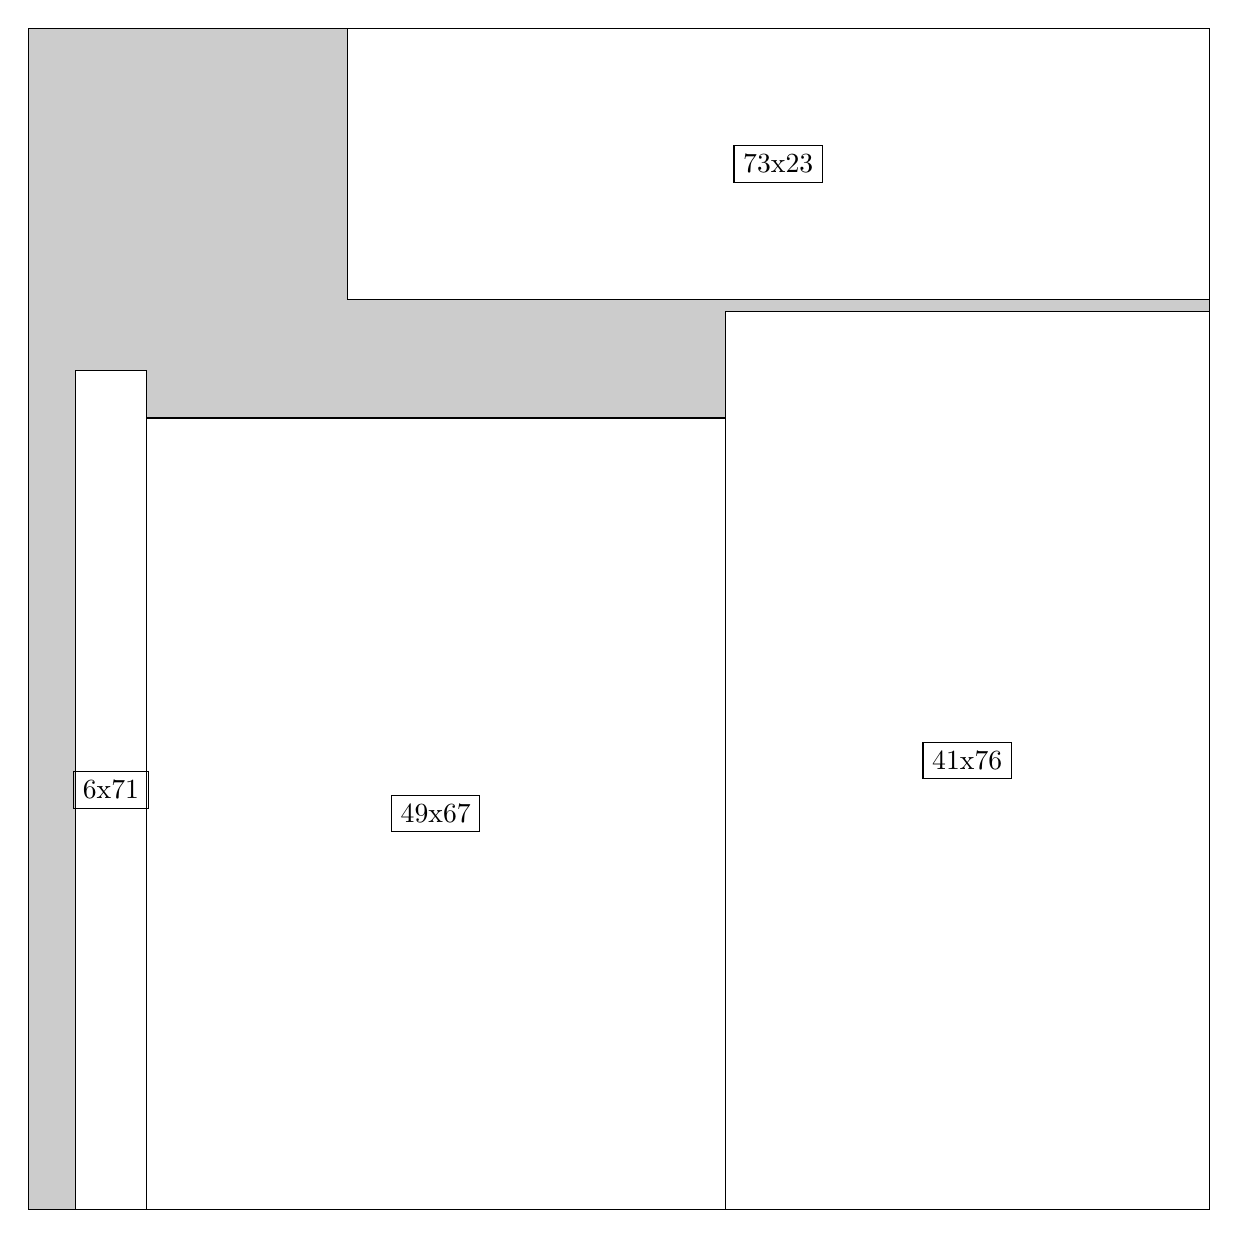
\begin{tikzpicture}[shorten >=1pt,scale=1.0,every node/.style={scale=1.0},->]
\tikzstyle{vertex}=[circle,fill=black!25,minimum size=14pt,inner sep=0pt]
\filldraw[fill=gray!40!white, draw=black] (0,0) rectangle (15.0,15.0);
\foreach \name/\x/\y/\w/\h in {41x76/8.85/0.0/6.1499999999999995/11.4,49x67/1.5/0.0/7.35/10.049999999999999,6x71/0.6/0.0/0.8999999999999999/10.65,73x23/4.05/11.549999999999999/10.95/3.4499999999999997}
\filldraw[fill=white!40!white, draw=black] (\x,\y) rectangle node[draw] (\name) {\name} ++(\w,\h);
\end{tikzpicture}


w =41 , h =76 , x =59 , y =0 , v =3116
\par
w =49 , h =67 , x =10 , y =0 , v =3283
\par
w =6 , h =71 , x =4 , y =0 , v =426
\par
w =73 , h =23 , x =27 , y =77 , v =1679
\par
\newpage


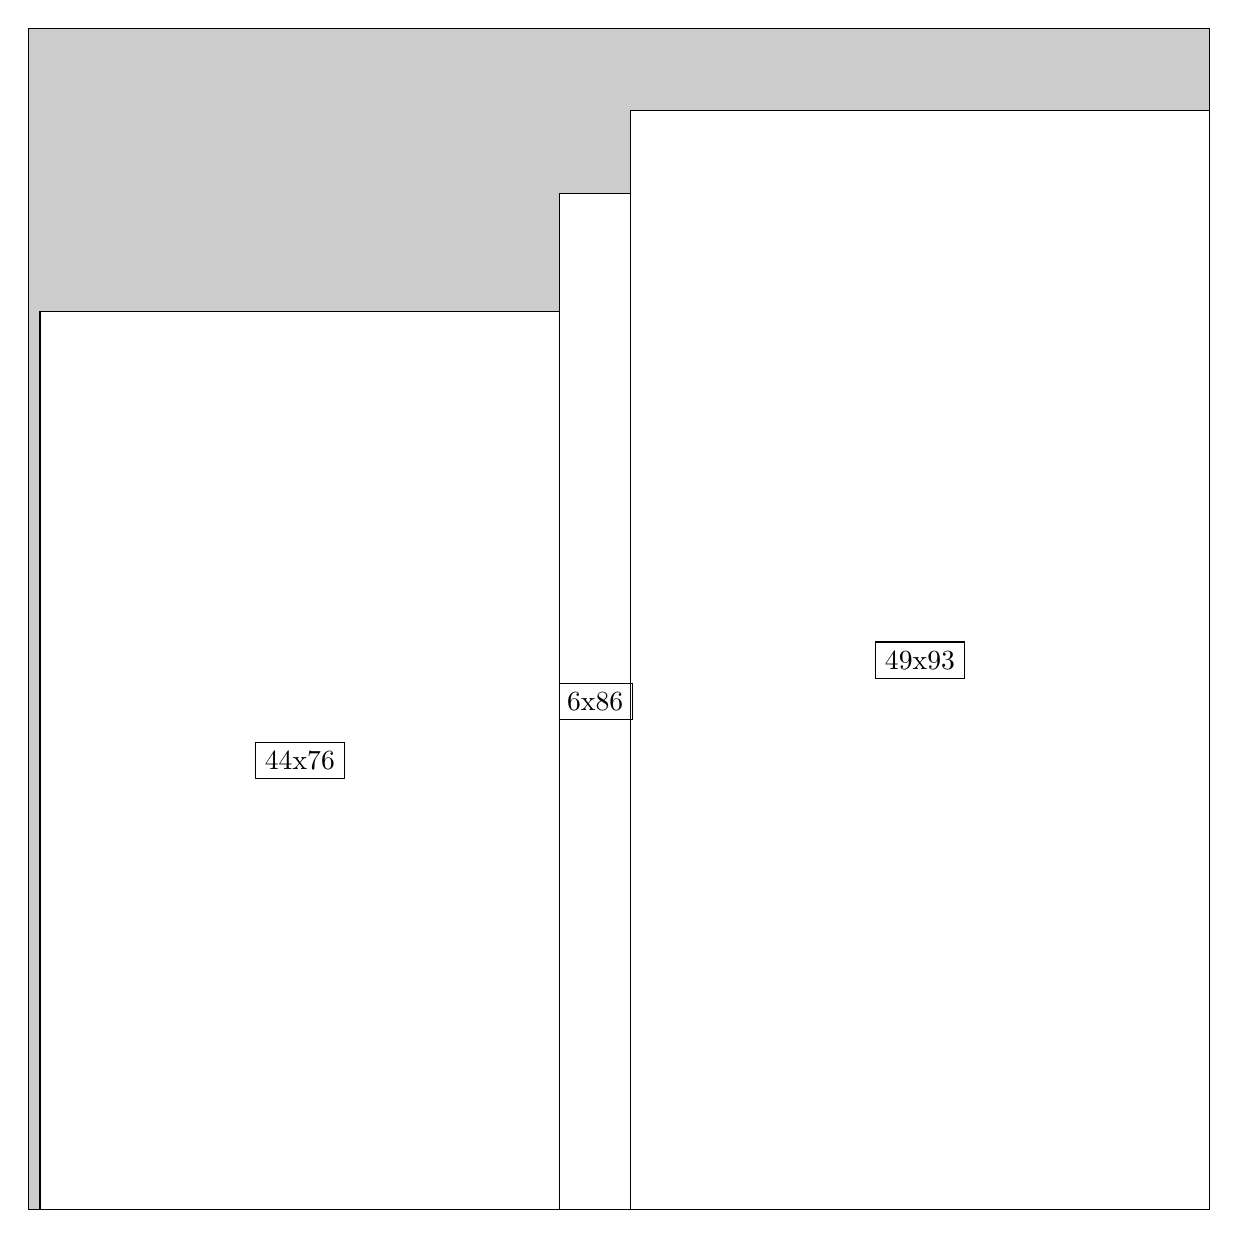
\begin{tikzpicture}[shorten >=1pt,scale=1.0,every node/.style={scale=1.0},->]
\tikzstyle{vertex}=[circle,fill=black!25,minimum size=14pt,inner sep=0pt]
\filldraw[fill=gray!40!white, draw=black] (0,0) rectangle (15.0,15.0);
\foreach \name/\x/\y/\w/\h in {49x93/7.6499999999999995/0.0/7.35/13.95,6x86/6.75/0.0/0.8999999999999999/12.9,44x76/0.15/0.0/6.6/11.4}
\filldraw[fill=white!40!white, draw=black] (\x,\y) rectangle node[draw] (\name) {\name} ++(\w,\h);
\end{tikzpicture}


w =49 , h =93 , x =51 , y =0 , v =4557
\par
w =6 , h =86 , x =45 , y =0 , v =516
\par
w =44 , h =76 , x =1 , y =0 , v =3344
\par
\newpage


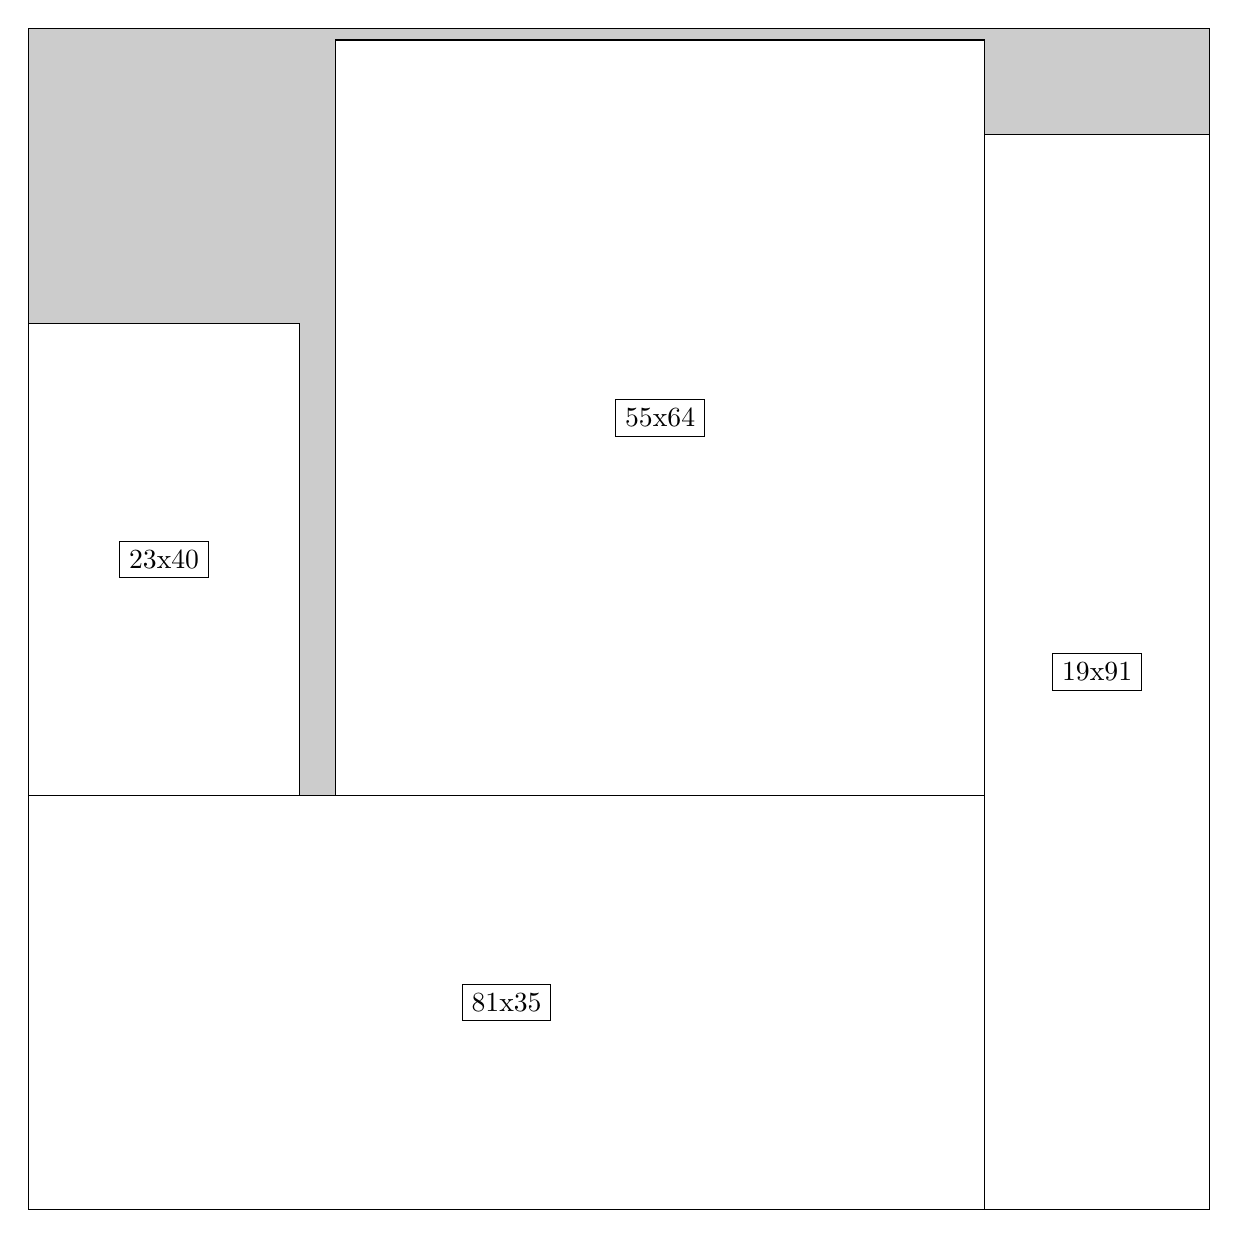
\begin{tikzpicture}[shorten >=1pt,scale=1.0,every node/.style={scale=1.0},->]
\tikzstyle{vertex}=[circle,fill=black!25,minimum size=14pt,inner sep=0pt]
\filldraw[fill=gray!40!white, draw=black] (0,0) rectangle (15.0,15.0);
\foreach \name/\x/\y/\w/\h in {19x91/12.15/0.0/2.85/13.65,81x35/0.0/0.0/12.15/5.25,55x64/3.9/5.25/8.25/9.6,23x40/0.0/5.25/3.4499999999999997/6.0}
\filldraw[fill=white!40!white, draw=black] (\x,\y) rectangle node[draw] (\name) {\name} ++(\w,\h);
\end{tikzpicture}


w =19 , h =91 , x =81 , y =0 , v =1729
\par
w =81 , h =35 , x =0 , y =0 , v =2835
\par
w =55 , h =64 , x =26 , y =35 , v =3520
\par
w =23 , h =40 , x =0 , y =35 , v =920
\par
\newpage


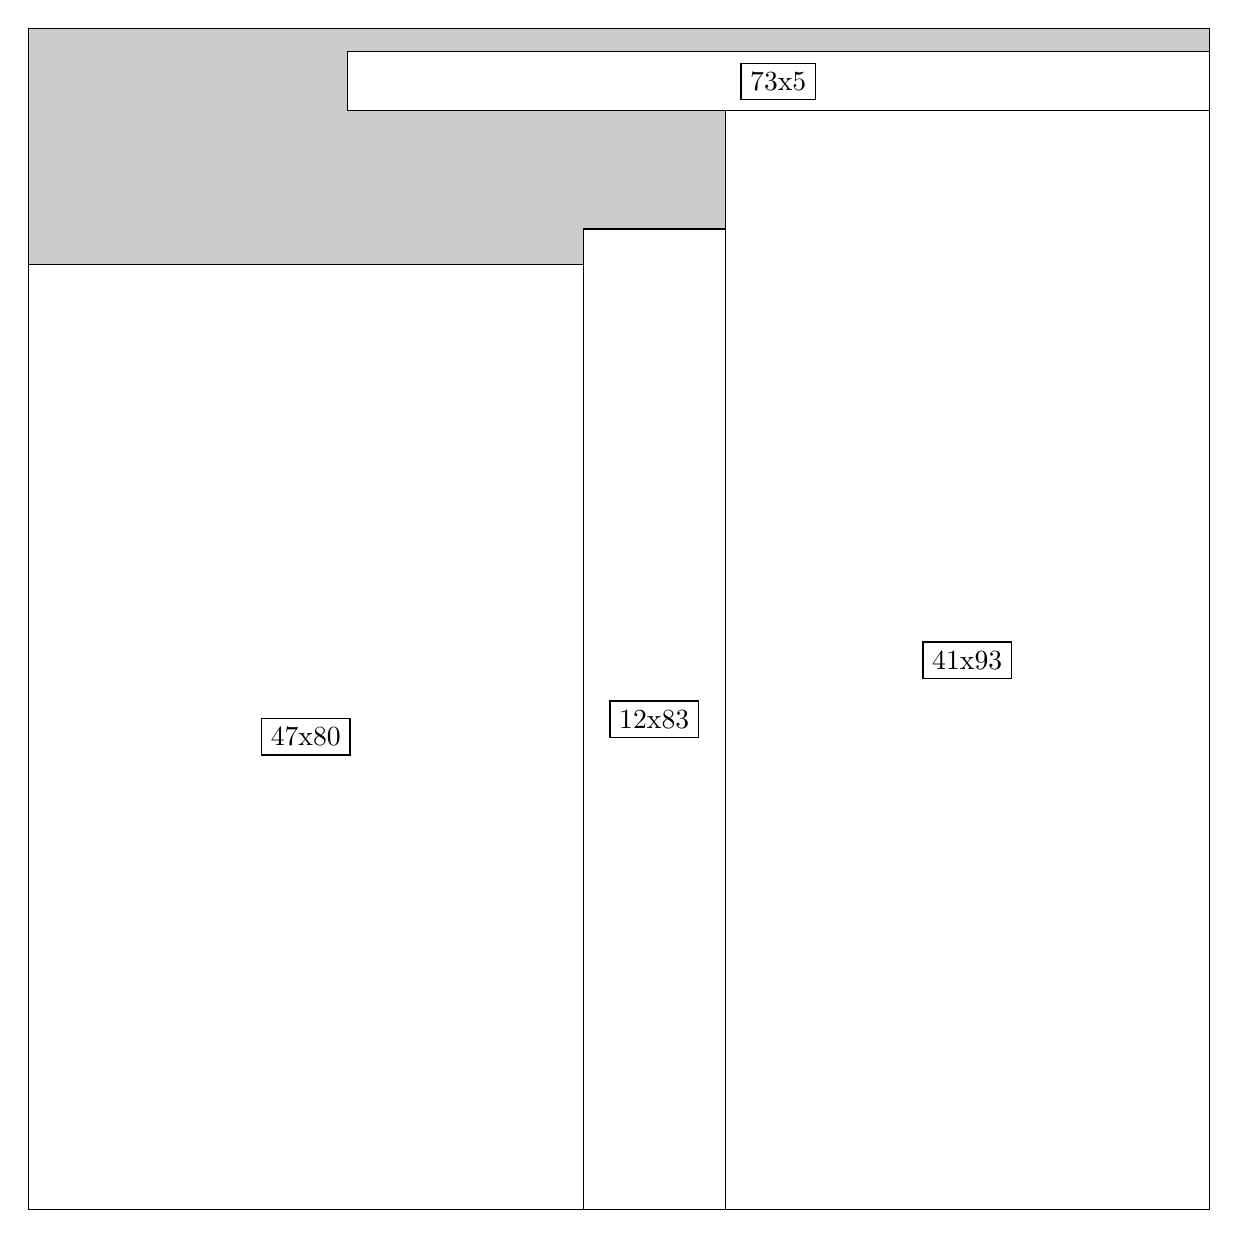
\begin{tikzpicture}[shorten >=1pt,scale=1.0,every node/.style={scale=1.0},->]
\tikzstyle{vertex}=[circle,fill=black!25,minimum size=14pt,inner sep=0pt]
\filldraw[fill=gray!40!white, draw=black] (0,0) rectangle (15.0,15.0);
\foreach \name/\x/\y/\w/\h in {41x93/8.85/0.0/6.1499999999999995/13.95,12x83/7.05/0.0/1.7999999999999998/12.45,47x80/0.0/0.0/7.05/12.0,73x5/4.05/13.95/10.95/0.75}
\filldraw[fill=white!40!white, draw=black] (\x,\y) rectangle node[draw] (\name) {\name} ++(\w,\h);
\end{tikzpicture}


w =41 , h =93 , x =59 , y =0 , v =3813
\par
w =12 , h =83 , x =47 , y =0 , v =996
\par
w =47 , h =80 , x =0 , y =0 , v =3760
\par
w =73 , h =5 , x =27 , y =93 , v =365
\par
\newpage


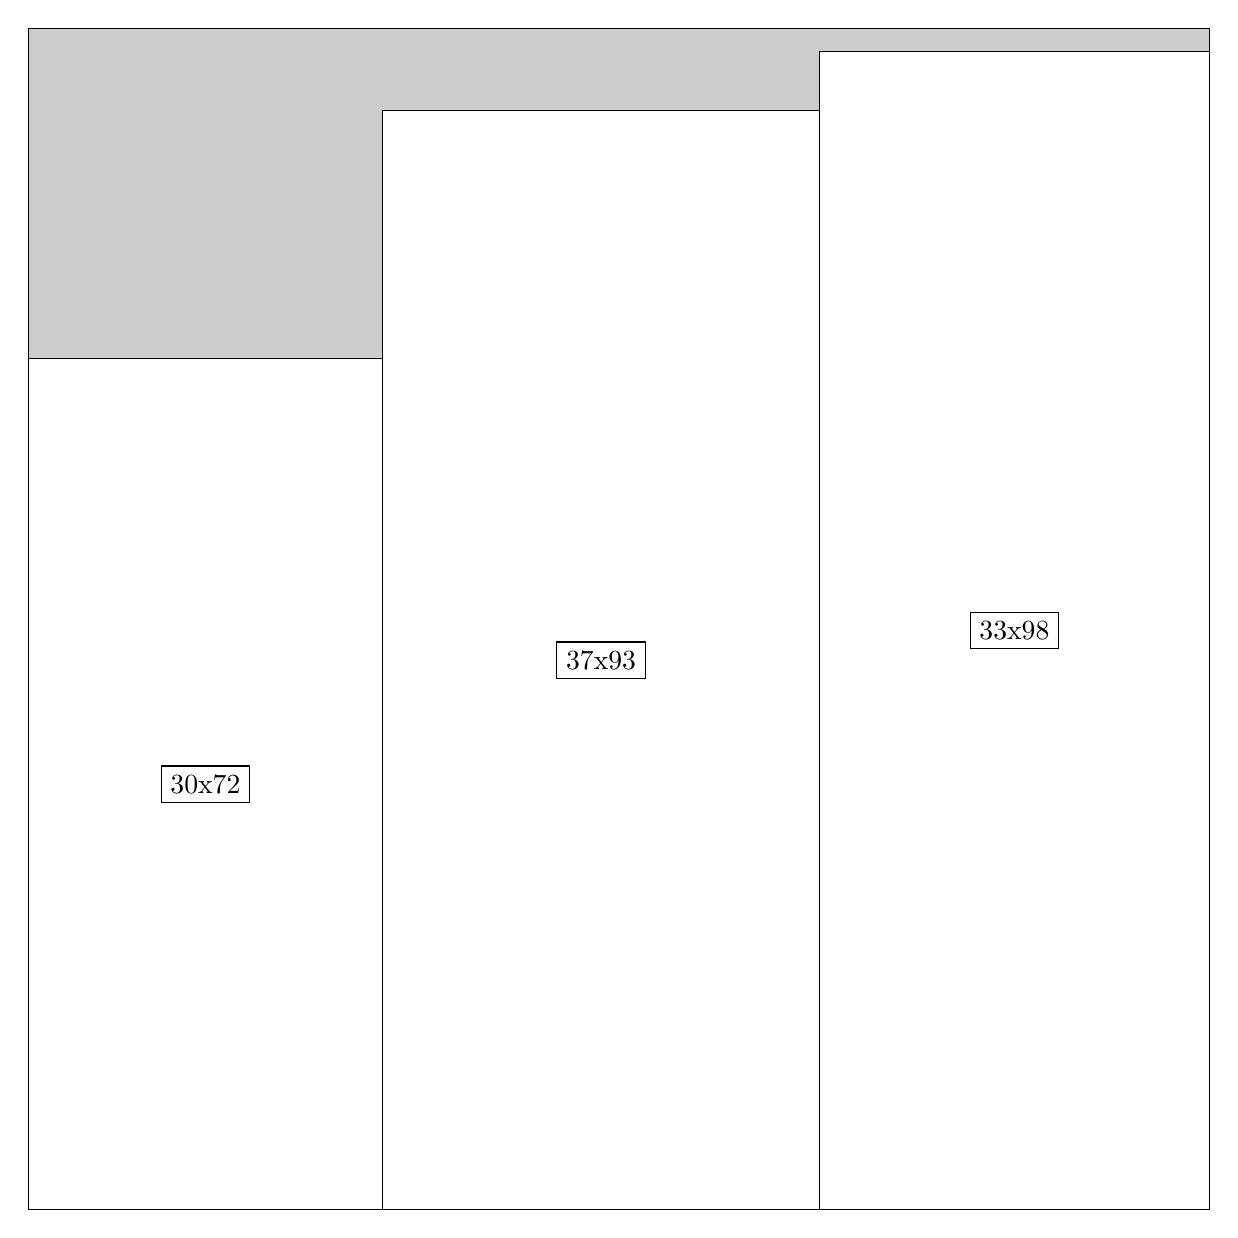
\begin{tikzpicture}[shorten >=1pt,scale=1.0,every node/.style={scale=1.0},->]
\tikzstyle{vertex}=[circle,fill=black!25,minimum size=14pt,inner sep=0pt]
\filldraw[fill=gray!40!white, draw=black] (0,0) rectangle (15.0,15.0);
\foreach \name/\x/\y/\w/\h in {33x98/10.049999999999999/0.0/4.95/14.7,37x93/4.5/0.0/5.55/13.95,30x72/0.0/0.0/4.5/10.799999999999999}
\filldraw[fill=white!40!white, draw=black] (\x,\y) rectangle node[draw] (\name) {\name} ++(\w,\h);
\end{tikzpicture}


w =33 , h =98 , x =67 , y =0 , v =3234
\par
w =37 , h =93 , x =30 , y =0 , v =3441
\par
w =30 , h =72 , x =0 , y =0 , v =2160
\par
\newpage


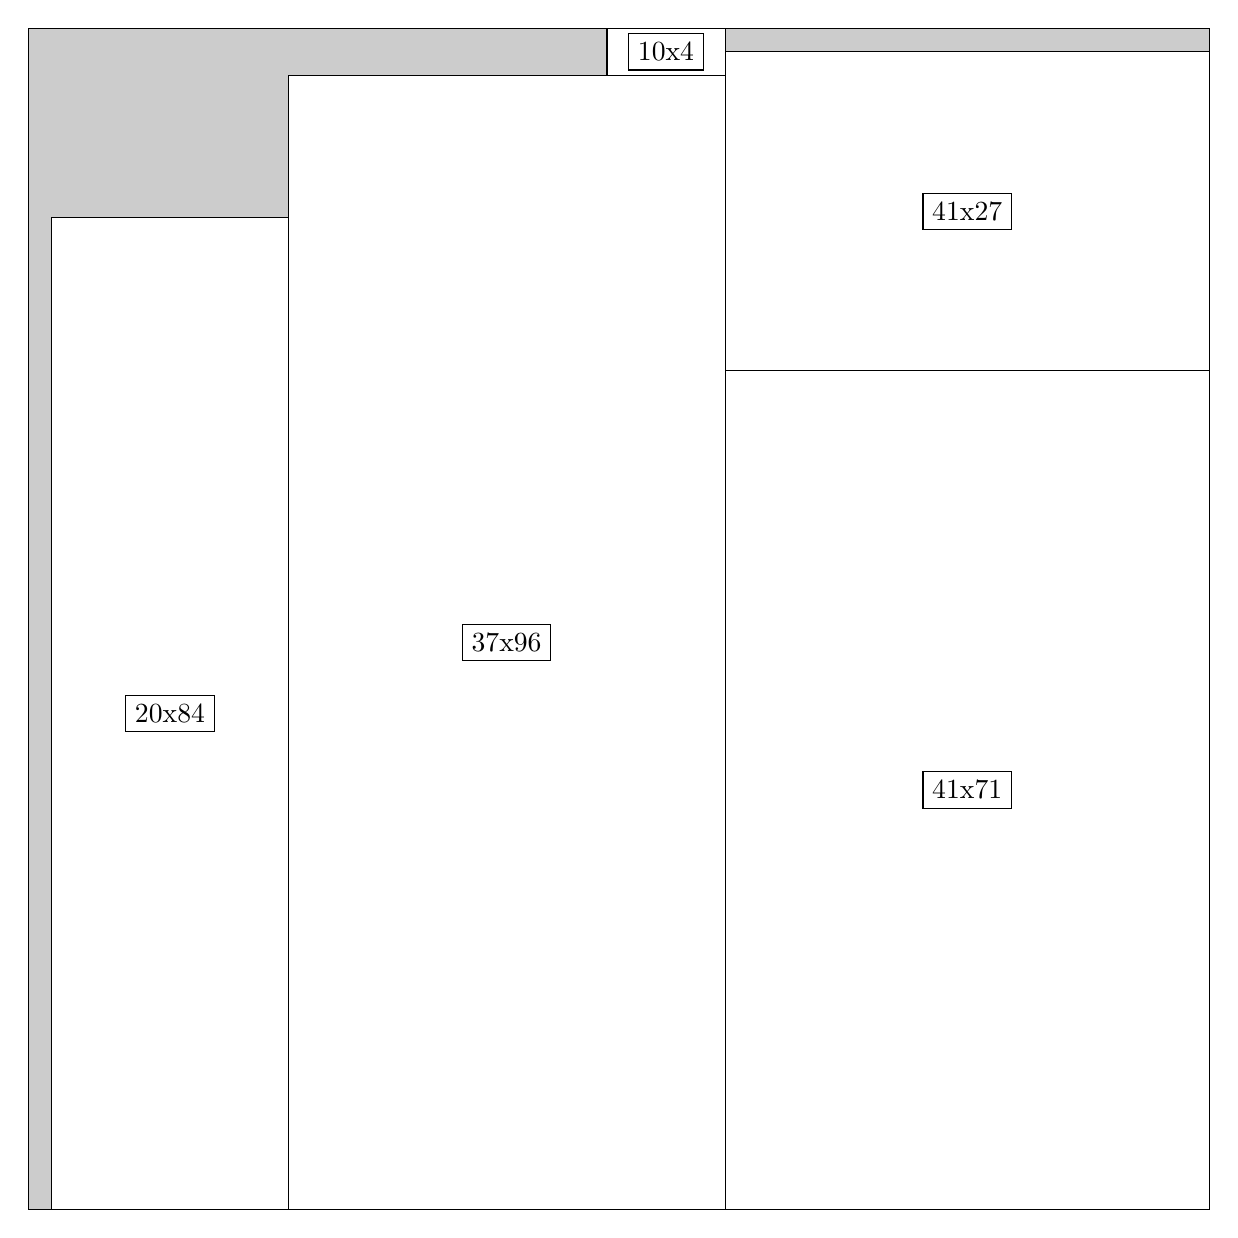
\begin{tikzpicture}[shorten >=1pt,scale=1.0,every node/.style={scale=1.0},->]
\tikzstyle{vertex}=[circle,fill=black!25,minimum size=14pt,inner sep=0pt]
\filldraw[fill=gray!40!white, draw=black] (0,0) rectangle (15.0,15.0);
\foreach \name/\x/\y/\w/\h in {41x71/8.85/0.0/6.1499999999999995/10.65,41x27/8.85/10.65/6.1499999999999995/4.05,37x96/3.3/0.0/5.55/14.399999999999999,10x4/7.35/14.399999999999999/1.5/0.6,20x84/0.3/0.0/3.0/12.6}
\filldraw[fill=white!40!white, draw=black] (\x,\y) rectangle node[draw] (\name) {\name} ++(\w,\h);
\end{tikzpicture}


w =41 , h =71 , x =59 , y =0 , v =2911
\par
w =41 , h =27 , x =59 , y =71 , v =1107
\par
w =37 , h =96 , x =22 , y =0 , v =3552
\par
w =10 , h =4 , x =49 , y =96 , v =40
\par
w =20 , h =84 , x =2 , y =0 , v =1680
\par
\newpage


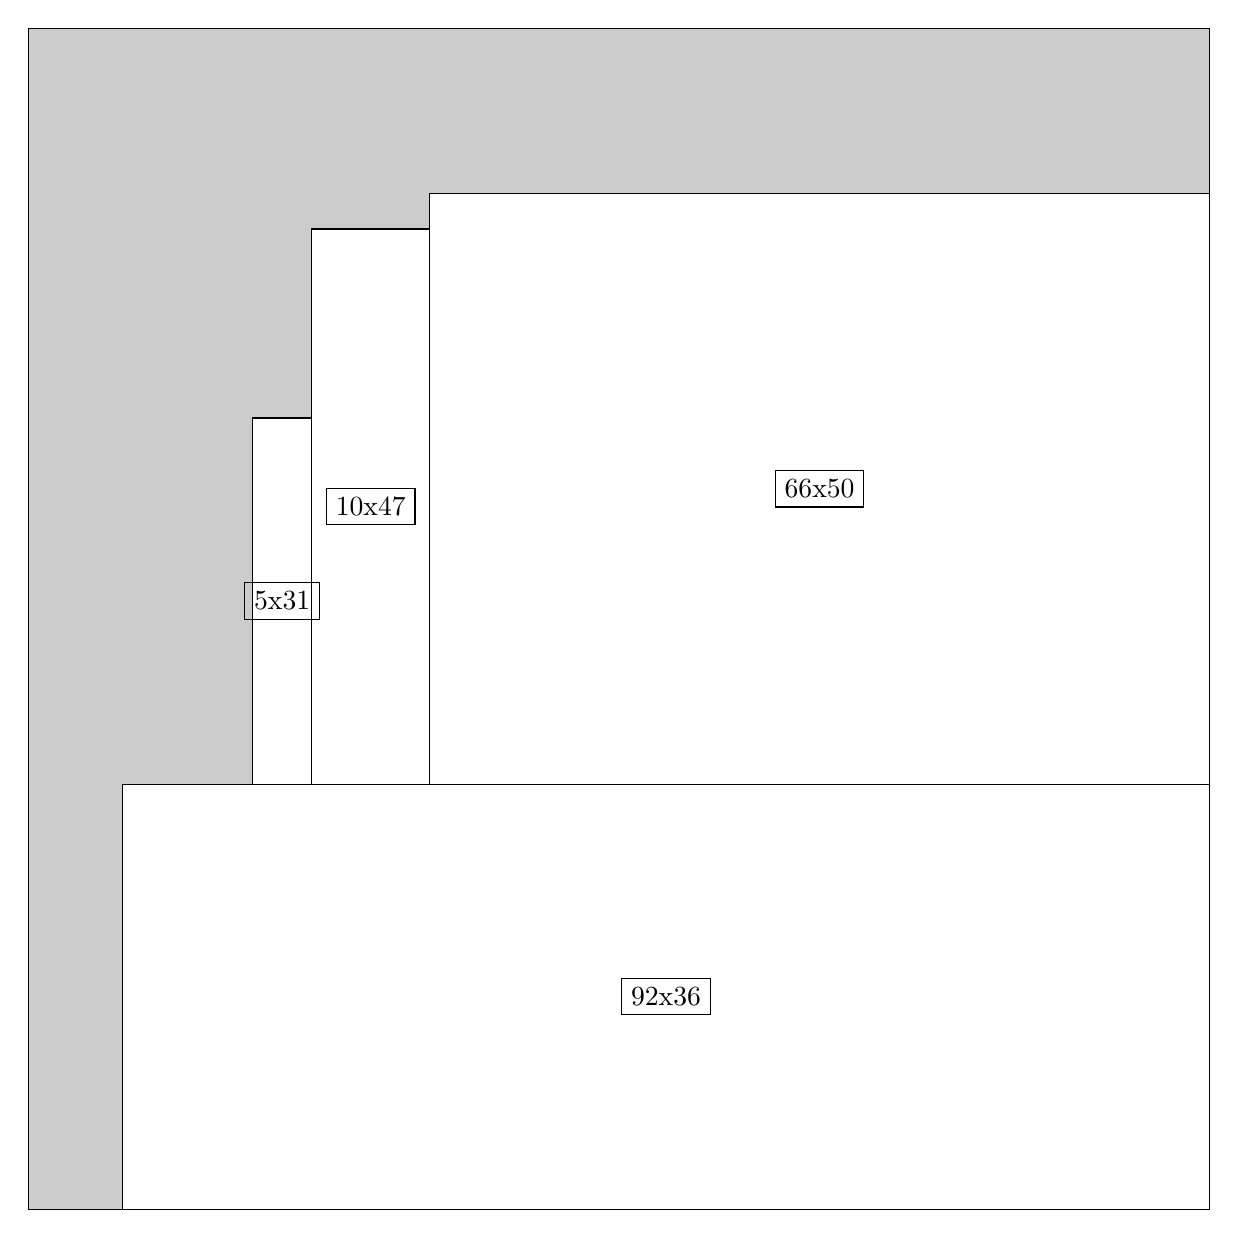
\begin{tikzpicture}[shorten >=1pt,scale=1.0,every node/.style={scale=1.0},->]
\tikzstyle{vertex}=[circle,fill=black!25,minimum size=14pt,inner sep=0pt]
\filldraw[fill=gray!40!white, draw=black] (0,0) rectangle (15.0,15.0);
\foreach \name/\x/\y/\w/\h in {92x36/1.2/0.0/13.799999999999999/5.3999999999999995,66x50/5.1/5.3999999999999995/9.9/7.5,10x47/3.5999999999999996/5.3999999999999995/1.5/7.05,5x31/2.85/5.3999999999999995/0.75/4.6499999999999995}
\filldraw[fill=white!40!white, draw=black] (\x,\y) rectangle node[draw] (\name) {\name} ++(\w,\h);
\end{tikzpicture}


w =92 , h =36 , x =8 , y =0 , v =3312
\par
w =66 , h =50 , x =34 , y =36 , v =3300
\par
w =10 , h =47 , x =24 , y =36 , v =470
\par
w =5 , h =31 , x =19 , y =36 , v =155
\par
\newpage


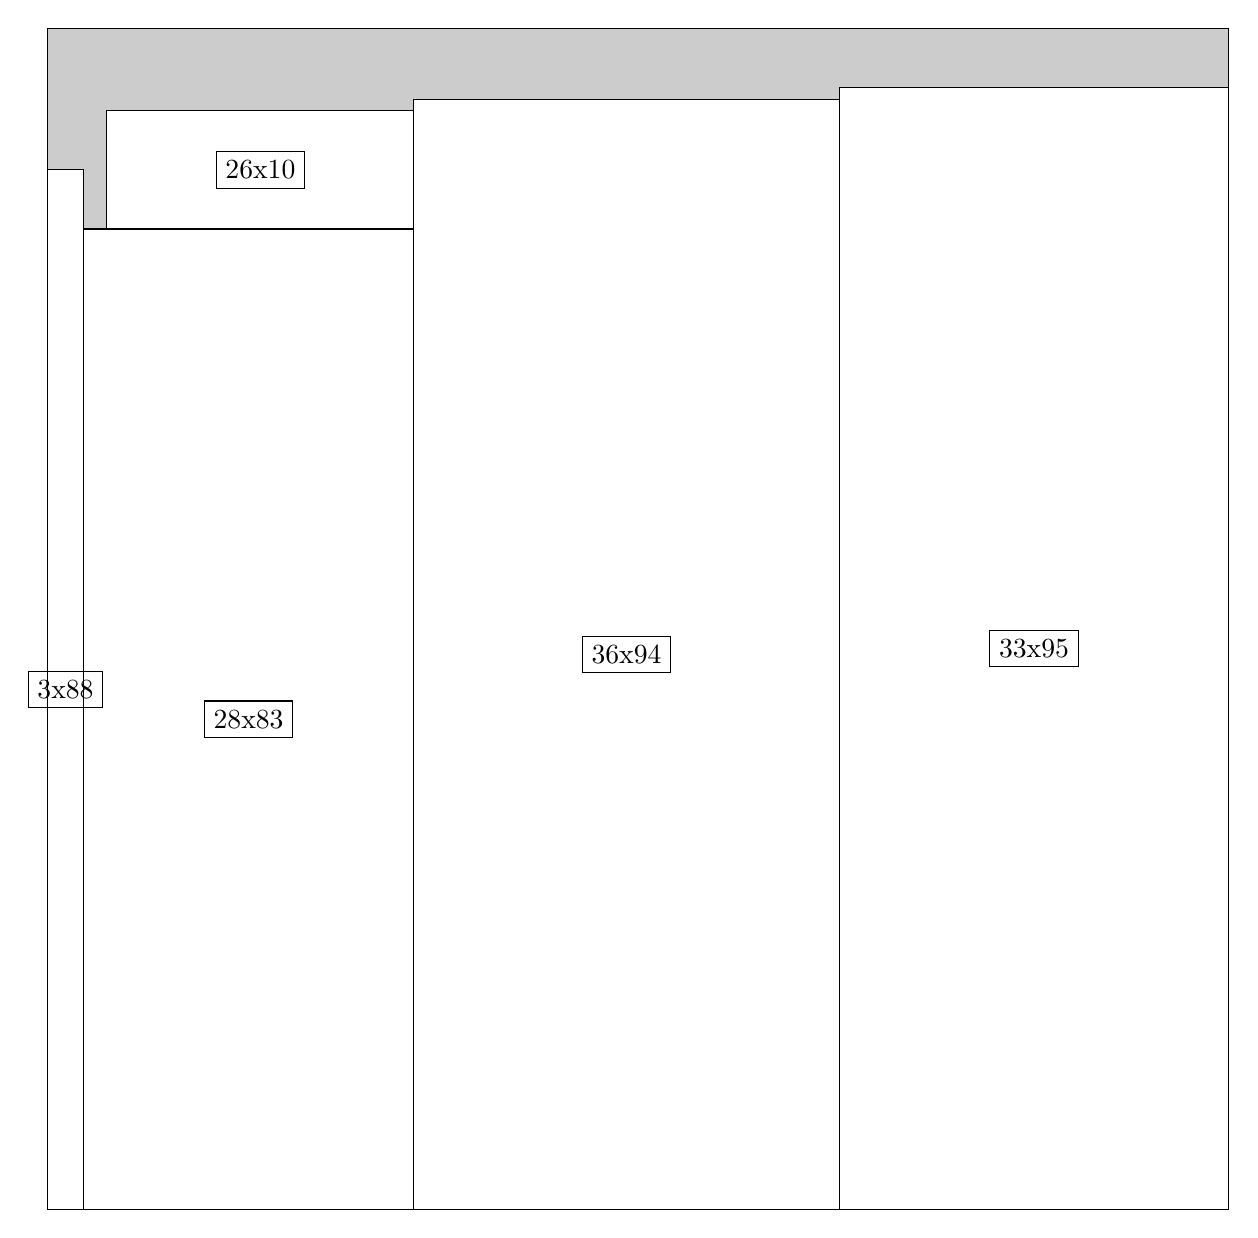
\begin{tikzpicture}[shorten >=1pt,scale=1.0,every node/.style={scale=1.0},->]
\tikzstyle{vertex}=[circle,fill=black!25,minimum size=14pt,inner sep=0pt]
\filldraw[fill=gray!40!white, draw=black] (0,0) rectangle (15.0,15.0);
\foreach \name/\x/\y/\w/\h in {33x95/10.049999999999999/0.0/4.95/14.25,36x94/4.6499999999999995/0.0/5.3999999999999995/14.1,28x83/0.44999999999999996/0.0/4.2/12.45,26x10/0.75/12.45/3.9/1.5,3x88/0.0/0.0/0.44999999999999996/13.2}
\filldraw[fill=white!40!white, draw=black] (\x,\y) rectangle node[draw] (\name) {\name} ++(\w,\h);
\end{tikzpicture}


w =33 , h =95 , x =67 , y =0 , v =3135
\par
w =36 , h =94 , x =31 , y =0 , v =3384
\par
w =28 , h =83 , x =3 , y =0 , v =2324
\par
w =26 , h =10 , x =5 , y =83 , v =260
\par
w =3 , h =88 , x =0 , y =0 , v =264
\par
\newpage


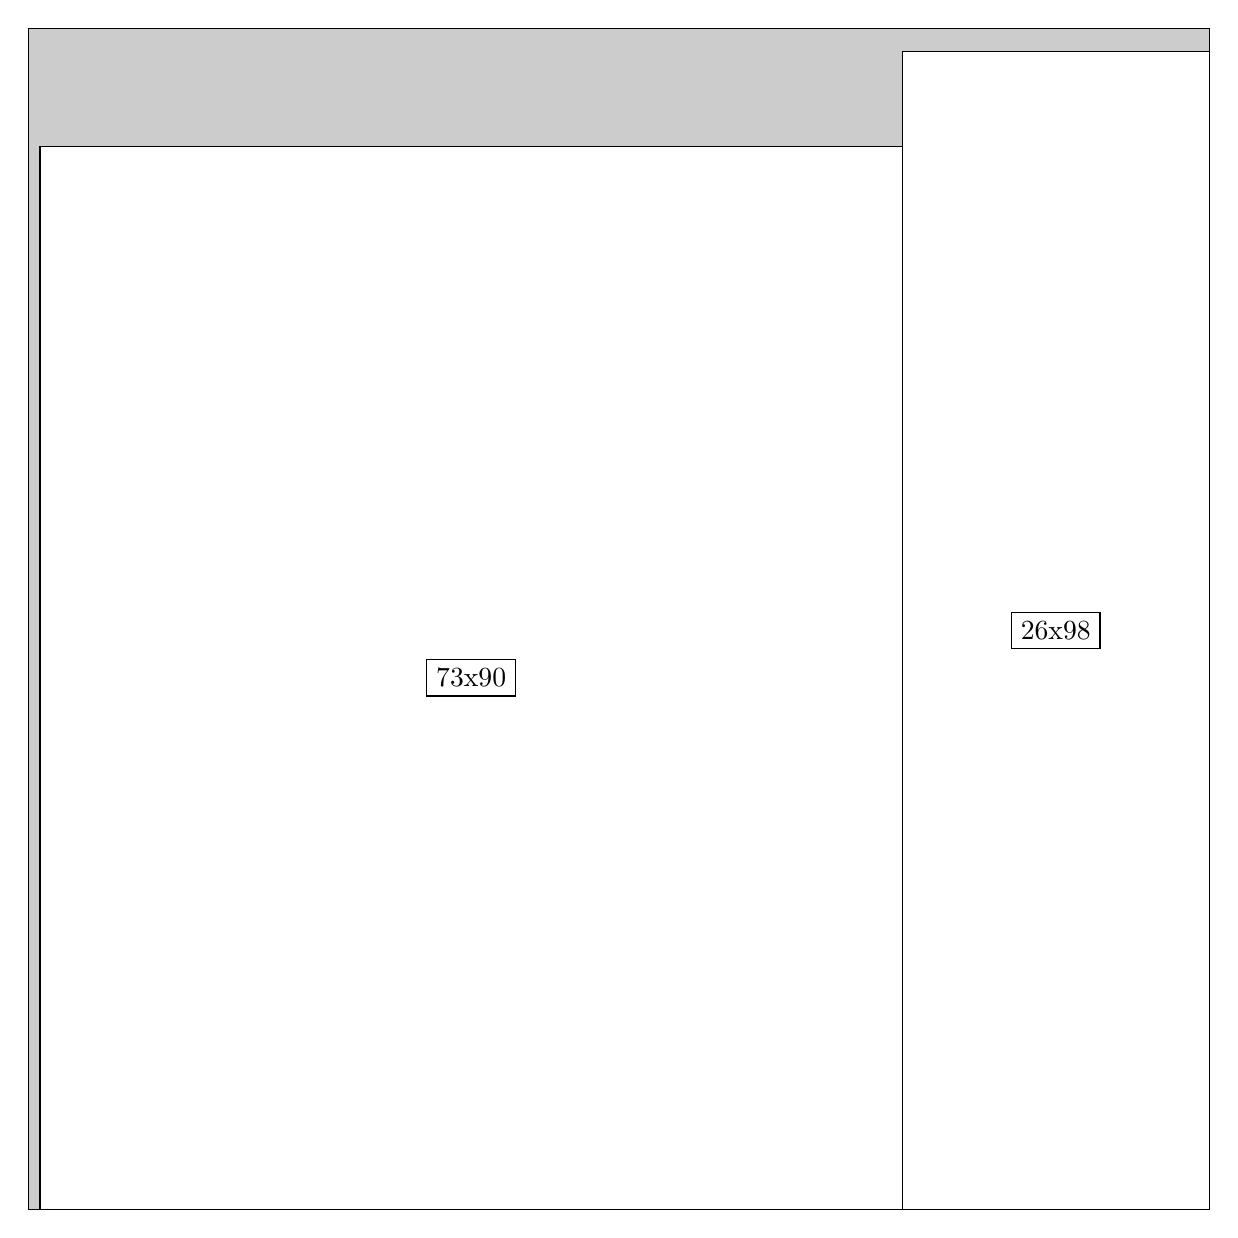
\begin{tikzpicture}[shorten >=1pt,scale=1.0,every node/.style={scale=1.0},->]
\tikzstyle{vertex}=[circle,fill=black!25,minimum size=14pt,inner sep=0pt]
\filldraw[fill=gray!40!white, draw=black] (0,0) rectangle (15.0,15.0);
\foreach \name/\x/\y/\w/\h in {26x98/11.1/0.0/3.9/14.7,73x90/0.15/0.0/10.95/13.5}
\filldraw[fill=white!40!white, draw=black] (\x,\y) rectangle node[draw] (\name) {\name} ++(\w,\h);
\end{tikzpicture}


w =26 , h =98 , x =74 , y =0 , v =2548
\par
w =73 , h =90 , x =1 , y =0 , v =6570
\par
\newpage


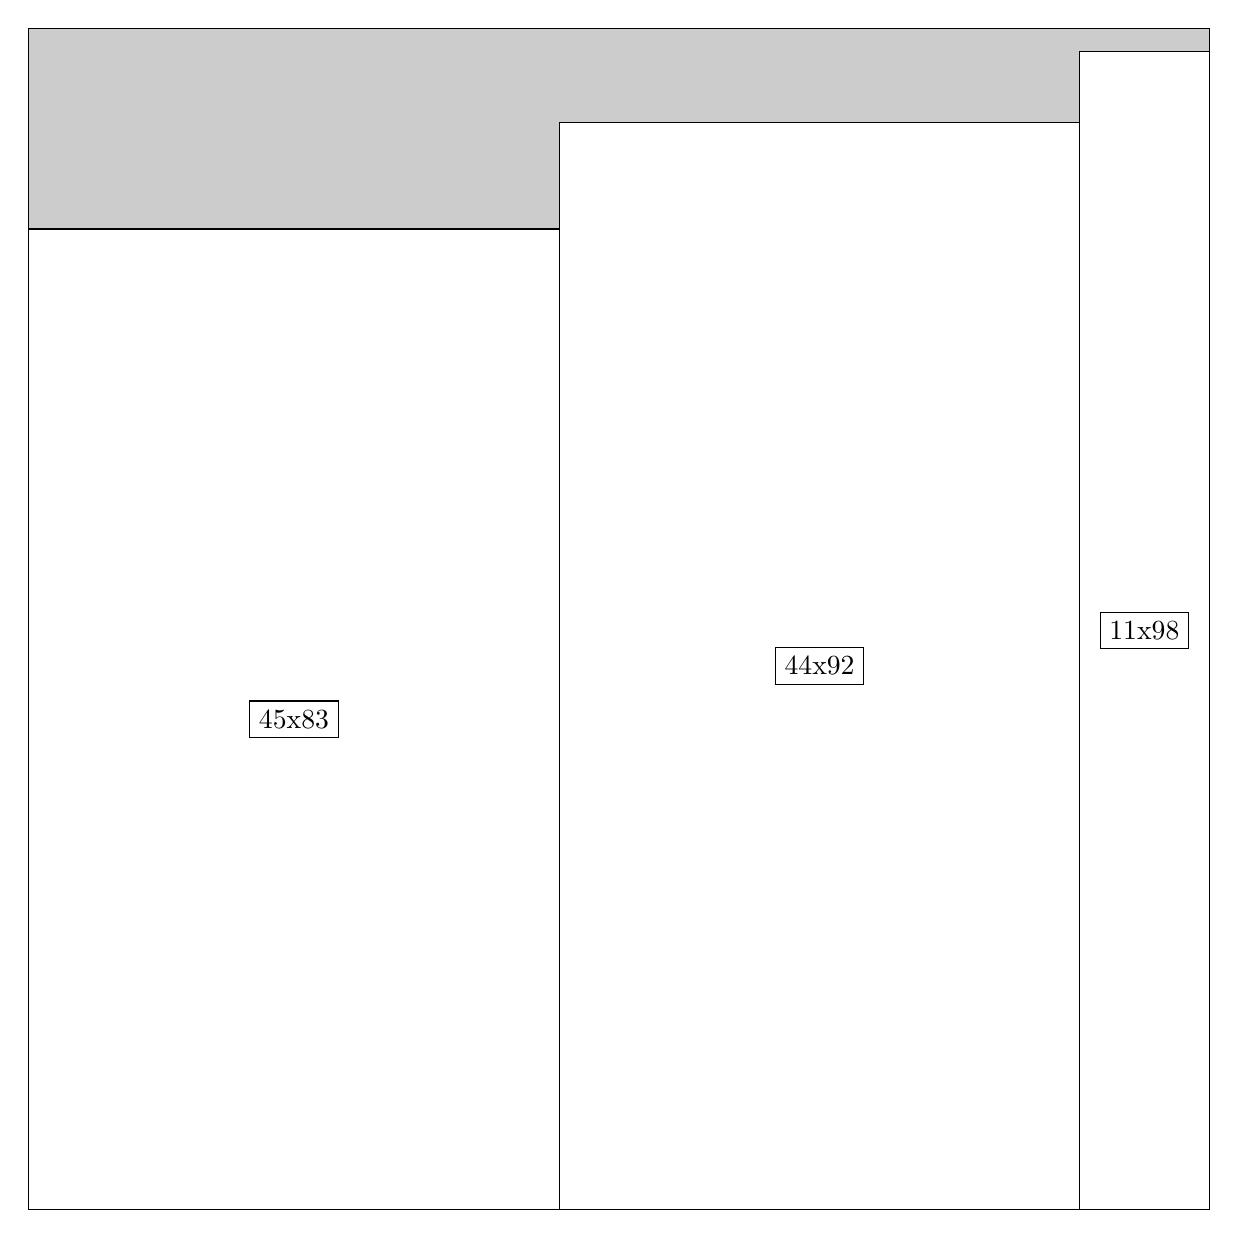
\begin{tikzpicture}[shorten >=1pt,scale=1.0,every node/.style={scale=1.0},->]
\tikzstyle{vertex}=[circle,fill=black!25,minimum size=14pt,inner sep=0pt]
\filldraw[fill=gray!40!white, draw=black] (0,0) rectangle (15.0,15.0);
\foreach \name/\x/\y/\w/\h in {11x98/13.35/0.0/1.65/14.7,44x92/6.75/0.0/6.6/13.799999999999999,45x83/0.0/0.0/6.75/12.45}
\filldraw[fill=white!40!white, draw=black] (\x,\y) rectangle node[draw] (\name) {\name} ++(\w,\h);
\end{tikzpicture}


w =11 , h =98 , x =89 , y =0 , v =1078
\par
w =44 , h =92 , x =45 , y =0 , v =4048
\par
w =45 , h =83 , x =0 , y =0 , v =3735
\par
\newpage


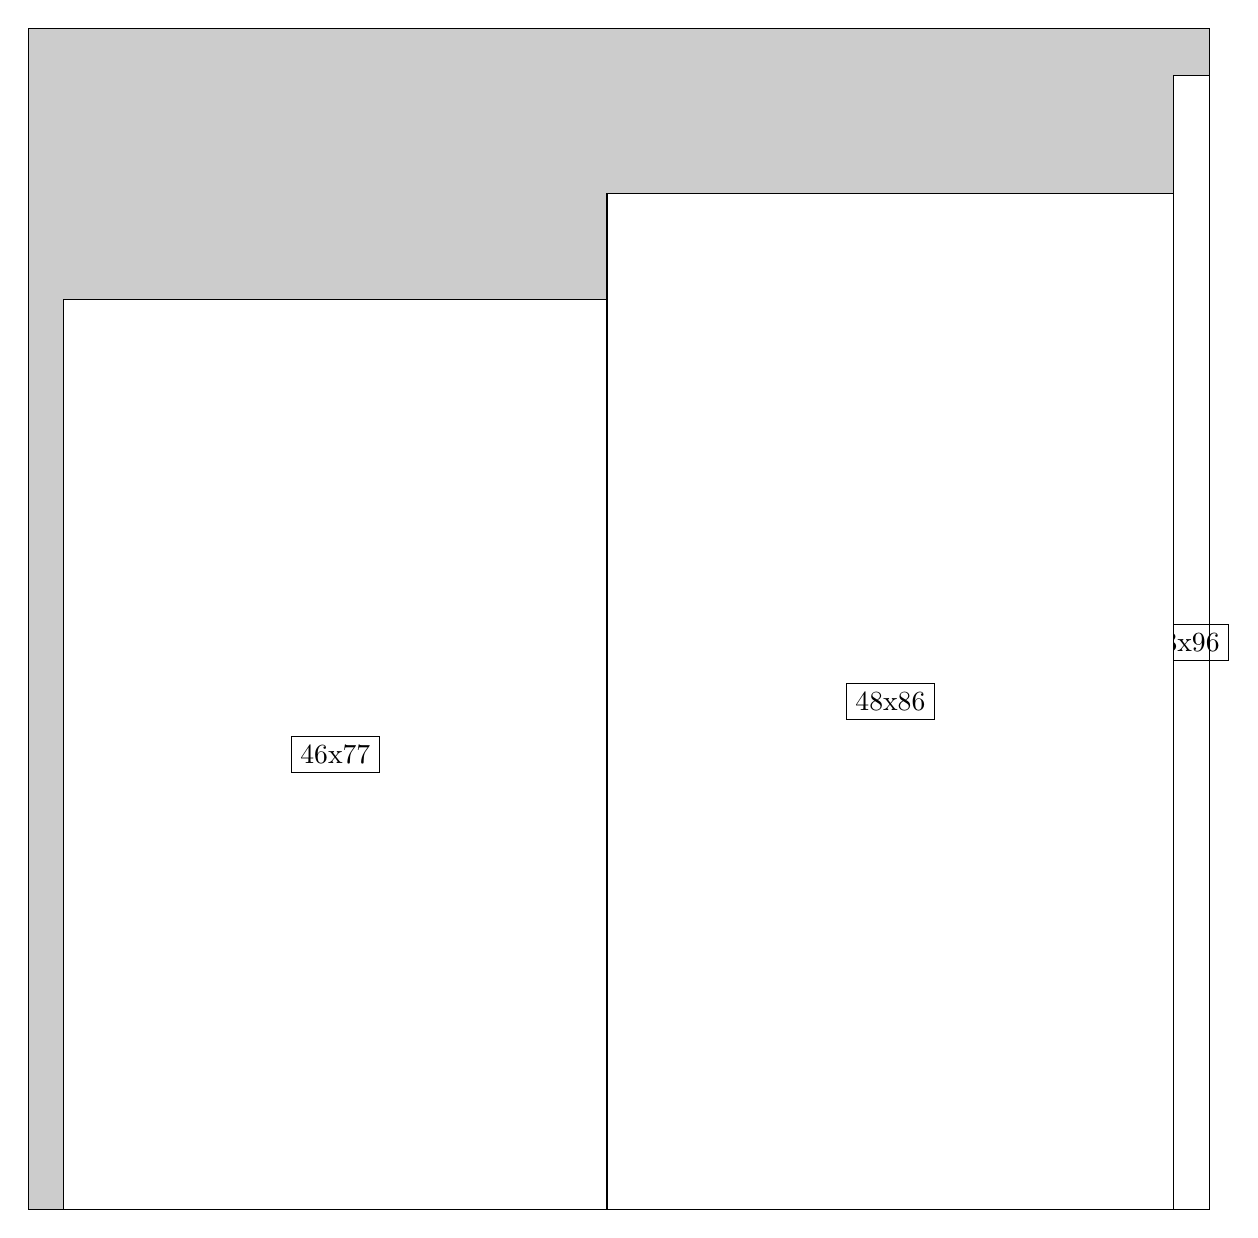
\begin{tikzpicture}[shorten >=1pt,scale=1.0,every node/.style={scale=1.0},->]
\tikzstyle{vertex}=[circle,fill=black!25,minimum size=14pt,inner sep=0pt]
\filldraw[fill=gray!40!white, draw=black] (0,0) rectangle (15.0,15.0);
\foreach \name/\x/\y/\w/\h in {3x96/14.549999999999999/0.0/0.44999999999999996/14.399999999999999,48x86/7.35/0.0/7.199999999999999/12.9,46x77/0.44999999999999996/0.0/6.8999999999999995/11.549999999999999}
\filldraw[fill=white!40!white, draw=black] (\x,\y) rectangle node[draw] (\name) {\name} ++(\w,\h);
\end{tikzpicture}


w =3 , h =96 , x =97 , y =0 , v =288
\par
w =48 , h =86 , x =49 , y =0 , v =4128
\par
w =46 , h =77 , x =3 , y =0 , v =3542
\par
\newpage


\end{document}